Det viser sig at mange tilfældige variable kan kategoriseres med en \emph{parametrisk} fordeling hvor pmf/pdf'en er bestemt ud fra én eller flere parametre. Her vil vi se på nogle af de mest almindelige, hvornår disse optræder i virkeligheden og hvilke statistikker, der karakteriserer dem. 
\subsection{Bernoulli fordelingen}
En diskret tilfældig variabel der er $1$ med sandsynlighed $p$ og $0$ med sandsynlighed $1-p$ for $p \in [0,1]$ kaldes en Bernoulli fordeling. Hvis $X$ følger en Bernoulli fordeling med parametren $p$ da er pmf'en:
\begin{align*}
p_X(x) = \begin{cases} p & x = 1 \\
1 - p & x = 0 
\end{cases},
\end{align*} 
og vi skriver $X \sim B(p)$ der betyder ``$X$ følger en Bernoulli fordeling med parameter $p$''. Vi har $E[X] = p$ og $\Var[x] = p(1-p)$. 
\begin{example}
En sygdom overføres mellem to personer med sandsynlighed $p = 0.25$.  \\ 
Hvis  $X(\text{``smitte overføres''}) = 1$ og $X(\text{``ingen smitte overføres''}) = 0$, da har vi $X \sim B(0.25)$ med forventet værdi $E[X] = 0.25$ og standardafvigelse $\Std[X] = \sqrt{(0.25)(1-0.25)} \approx 0.43$. Man siger så at smitte overføres forventeligt $25\%$ af gangene med en standardafvigelse på $43\%$ altså $25\% \pm 43\%$. Se \cite[111-112]{olofsson2012} for mere om Bernoulli fordelingen. 
\end{example}
\subsection{Uniform fordeling}
Hvis en tilfældig variabel har lige stor sandsynlighed for alle udfald i et interval kaldes den uniform. I terning eksemplet introduceret i eksempel \ref{ex:terning1} følger $X$ er en diskret tilfældig variabel med en uniform fordelingen for udfaldene $1$ til $6$. Uniforme fordelinger ses dog typisk for kontinuerte tilfældige variable som i eksempel \ref{ex:unif1}. Hvis $X$ følger en uniform fordelingen inden for intervallet $[a,b]$ da gælder at:
\begin{align*}
p_X(x) = \frac{1}{b-a}, \quad x \in [a,b],
\end{align*}
og vi skriver $X \sim \text{unif}(a,b)$. Vi har $E[X] = (a+b)/2$ og $\Var[X] = (b-a)^2/12$. Se \cite[90-92]{olofsson2012} for mere om den uniforme fordeling. 
\subsection{Poisson fordelingen}
Poisson fordelingen er en diskret fordeling og er vigtig inden for simulering, da den ofte ses for tilfældige variable, der beskriver antallet af uforudsigelige hændelser inden for en tidsperiode. Typiske eksempler er antallet af jordskælv, bilulykker, besøg på en hjemmeside og  antallet af stavefejl i en P1 rapport. Den originale brug af Poisson fordelingen var af Siméon Poisson, der opfandt fordelingen til at beskrive antallet af Preussiske soldater, der blev sparket ihjel af deres hest i det 19. århundrede. Det tilfældige element er vigtigt for Poisson fordelingen. Et eksempel som ankomsttidspunkter for busser vil derfor ikke være Poisson fordelt da tidsplanen fjerner det tilfældige element. Poisson fordelingen er karakteriseret ud fra parameteren $\lambda$ og har mulige udfald i de ikke negative heltal. Hvis $X$ følger en Poisson fordeling med parameter $\lambda$ da gælder at:
\begin{align*}
p_X(x) = e^{-\lambda}\frac{\lambda^x}{x!}, \quad x = 0,1,2,\dots \ ,
\end{align*}
og vi skriver $X \sim \text{Poi}(\lambda)$ (se figur \ref{fig:poiss}). Poisson fordelingen har den specielle egenskab at variansen er lig den forventede værdi som er $E[X] = \lambda$ og $\Var[X] = \lambda$. Se \cite[117-120]{olofsson2012} for mere om Poisson fordelingen. 
\begin{example}
I figur \ref{fig:horse} ses nævnte eksempel med antallet af omkomne Preussiske soldater. Her sammenlignes et normaliseret histogram med Poisson fordelingen for $\lambda = 0.61$, og det ses at fordelingen passer godt. 
\end{example}
\begin{figure}
\centering
\begin{minipage}[b][][b]{.45\textwidth}
\centering
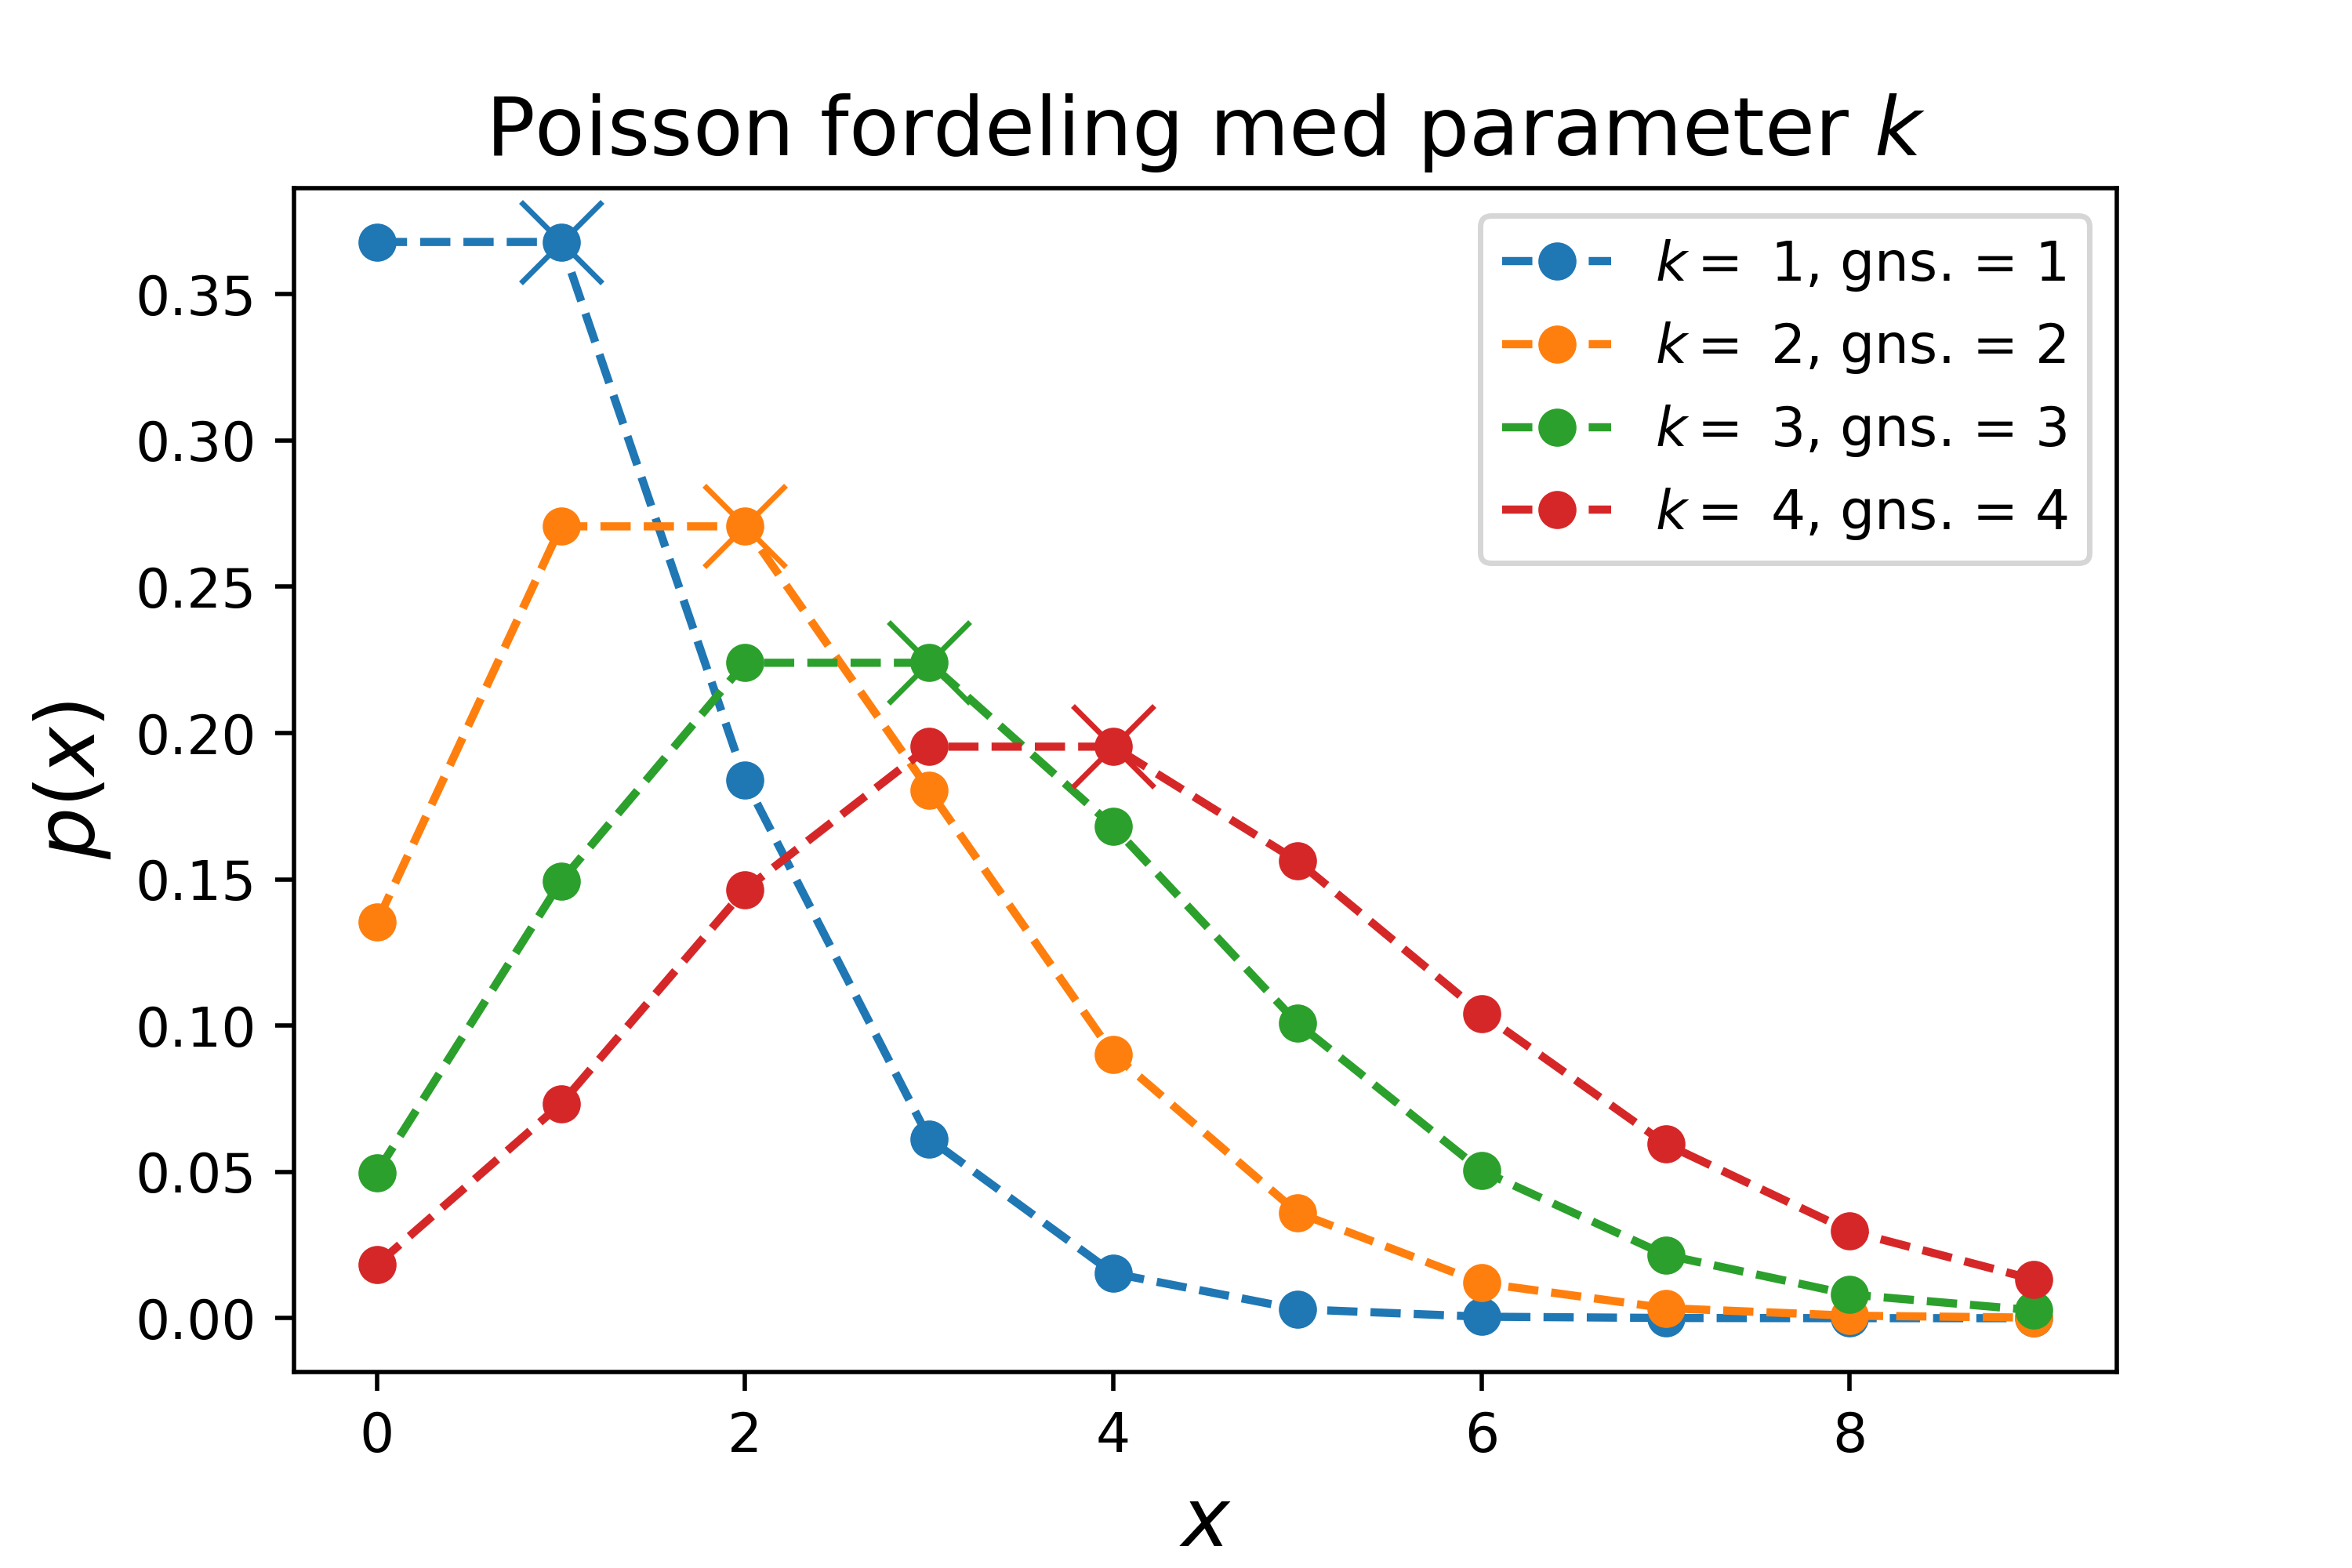
\includegraphics[width = \textwidth]{poiss_dist.png}
\caption{Poisson fordeling med forskellige parmetre $\lambda$. Stjernerne markerer forventet værdi.} \label{fig:poiss}
\end{minipage}
\begin{minipage}[b][][b]{.45\textwidth}
\centering
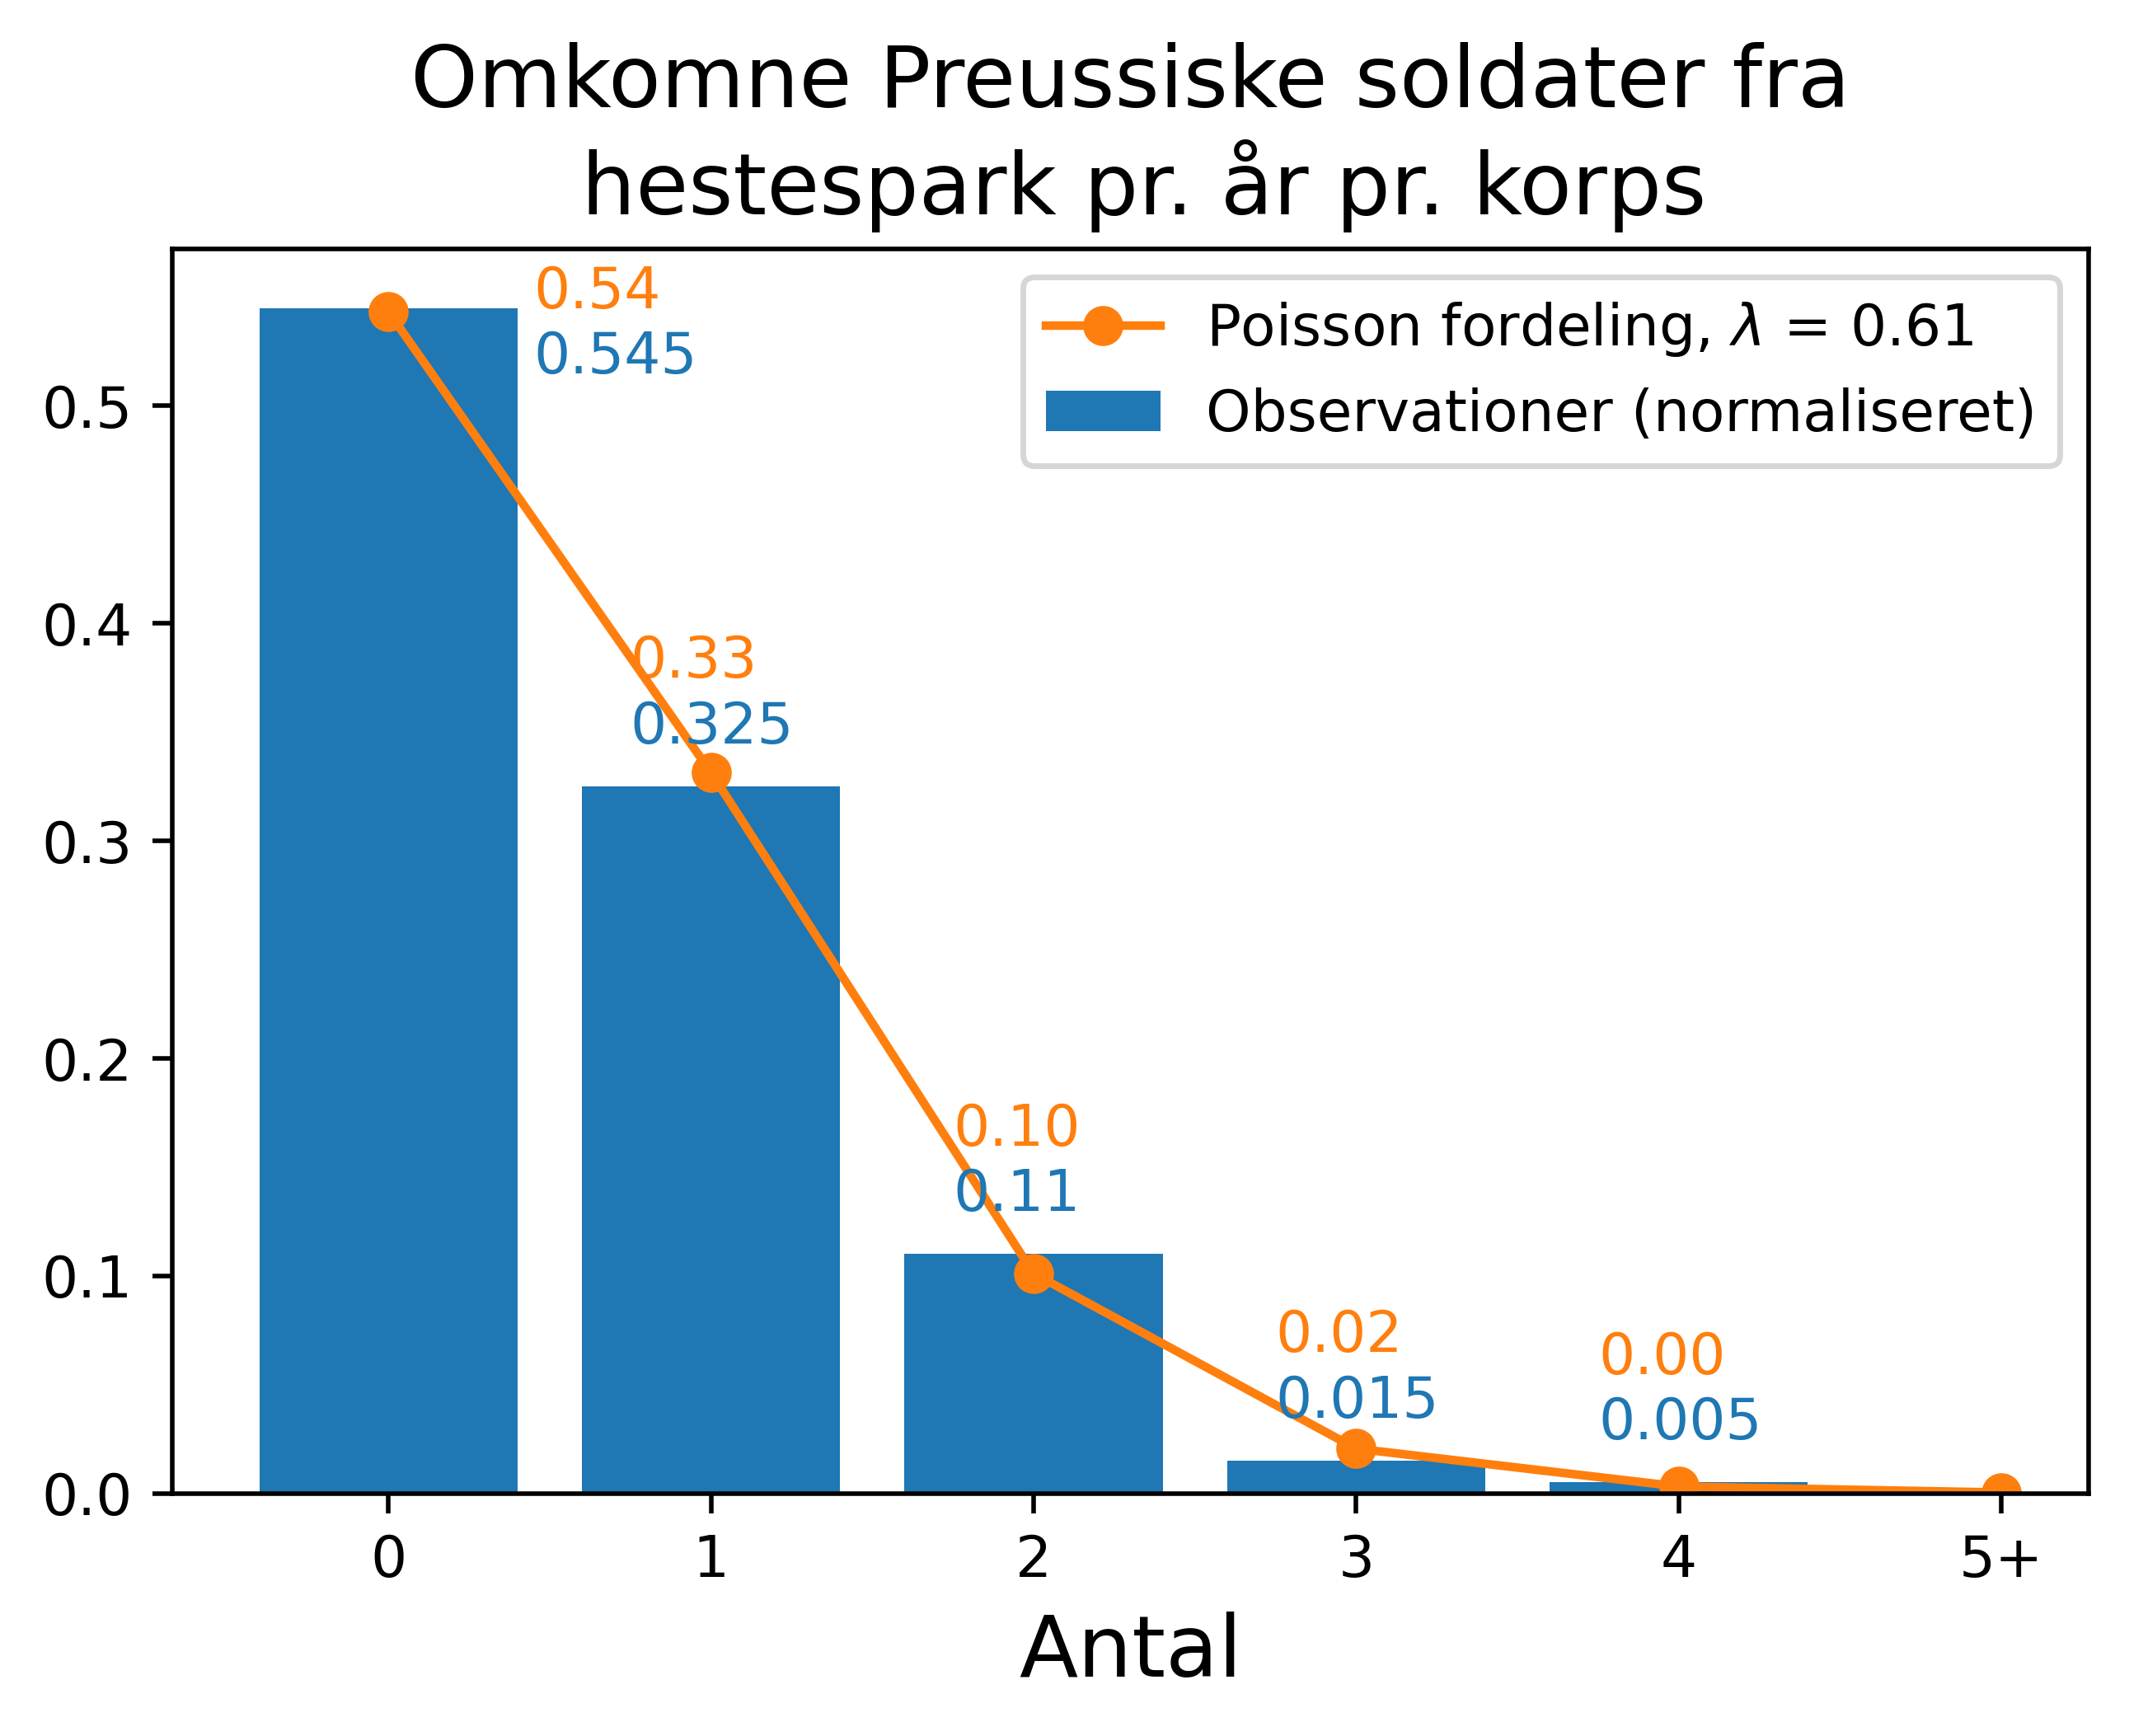
\includegraphics[width = \textwidth]{poiss_example.png}
\caption{Data: \cite{horse}\\ {\color{white}.}} \label{fig:horse}
\end{minipage}
\end{figure}
\subsection{Eksponentielfordeling}
Eksponentielfordelingen er en kontinuert fordeling, som også er vigtig inden for simulering, da den kan bruges til at modellere tiden mellem tilfældige hændelser. Dette kan være jordskælv, ankomst af kunder i en butik og antal tegn inden næste stavefejl i en P1 rapport. Eksponentielfordelingen har egenskaben at være \emph{hukommelsesløs}. Hukommelsesløse tilfældige variable \emph{ældes ikke} i den forstand at sandsynligheden for overlevelse endnu et stykke tid ikke afhænger af nuværende alder. Formelt skrives den hukommelsesløse egenskab for en tilfældig variabel $X$ som: 
\begin{align*}
P(X > x + y \text{ givet } X > y) = P(X > x)
\end{align*}
\begin{example} \label{ex:car1}
I et vejkryds på landet ankommer der en bil en gang i timen gennemsnitligt. Dette vil være en hukommelsesløs process da sandsynligheden for at der ikke kommer en ny bil efter eksempelvis $20$ minutter givet at der ikke er kommet en bil de første $10$ minutter er det samme som sandsynligheden for at der ikke kommer en ny bil efter $10$ minutter. 
\end{example}
Det viser sig at tilfældige variable med den hukommelsesløse egenskab nødvendigvis følger eksponentielfordelingen. Hvis $X$ følger en eksponentielfordeling med parameter $\lambda$ da er pdf'en:
\begin{align*}
p_X(x) = \lambda e^{-\lambda x}, \quad x \geq 0,
\end{align*}
og vi skriver $X \sim \exp(\lambda)$ (se figur \ref{fig:expnorm}). Vi har $E[X] = 1/\lambda$ og $\Var[X] = 1/\lambda^2$, som giver en fortolkning for $\lambda$ der kan refereres til som \emph{fejlraten}. Se \cite[123-127]{olofsson2012} for mere om eksponentielfordelingen. 
\begin{example} \label{ex:car2}
Hvis $T$ måler tiden i sekunder (s) mellem ankomsten af biler i eksempel \ref{ex:car1}, da vil $T$ modelleres godt som en eksponentielfordeling med parameter $\lambda = 1/60^2$ s$^{-1}$ og vi skriver $T \sim \exp(1/60^{2} \text{ s}^{-1})$. 
\end{example}
Den vågne læser har måske bemærket at der er en sammenhæng mellem eksponentielfordelingen, der modellerer tiden mellem tilfældige hændelser, og Poisson fordelingen der måler antallet af tilfældige hændelser inden for en tidsperiode. Denne sammenhæng vil blive belyst i afsnit \ref{sec:pointprocess}. 
\begin{figure}
\centering
\begin{minipage}[b][][b]{.45\textwidth}
\centering
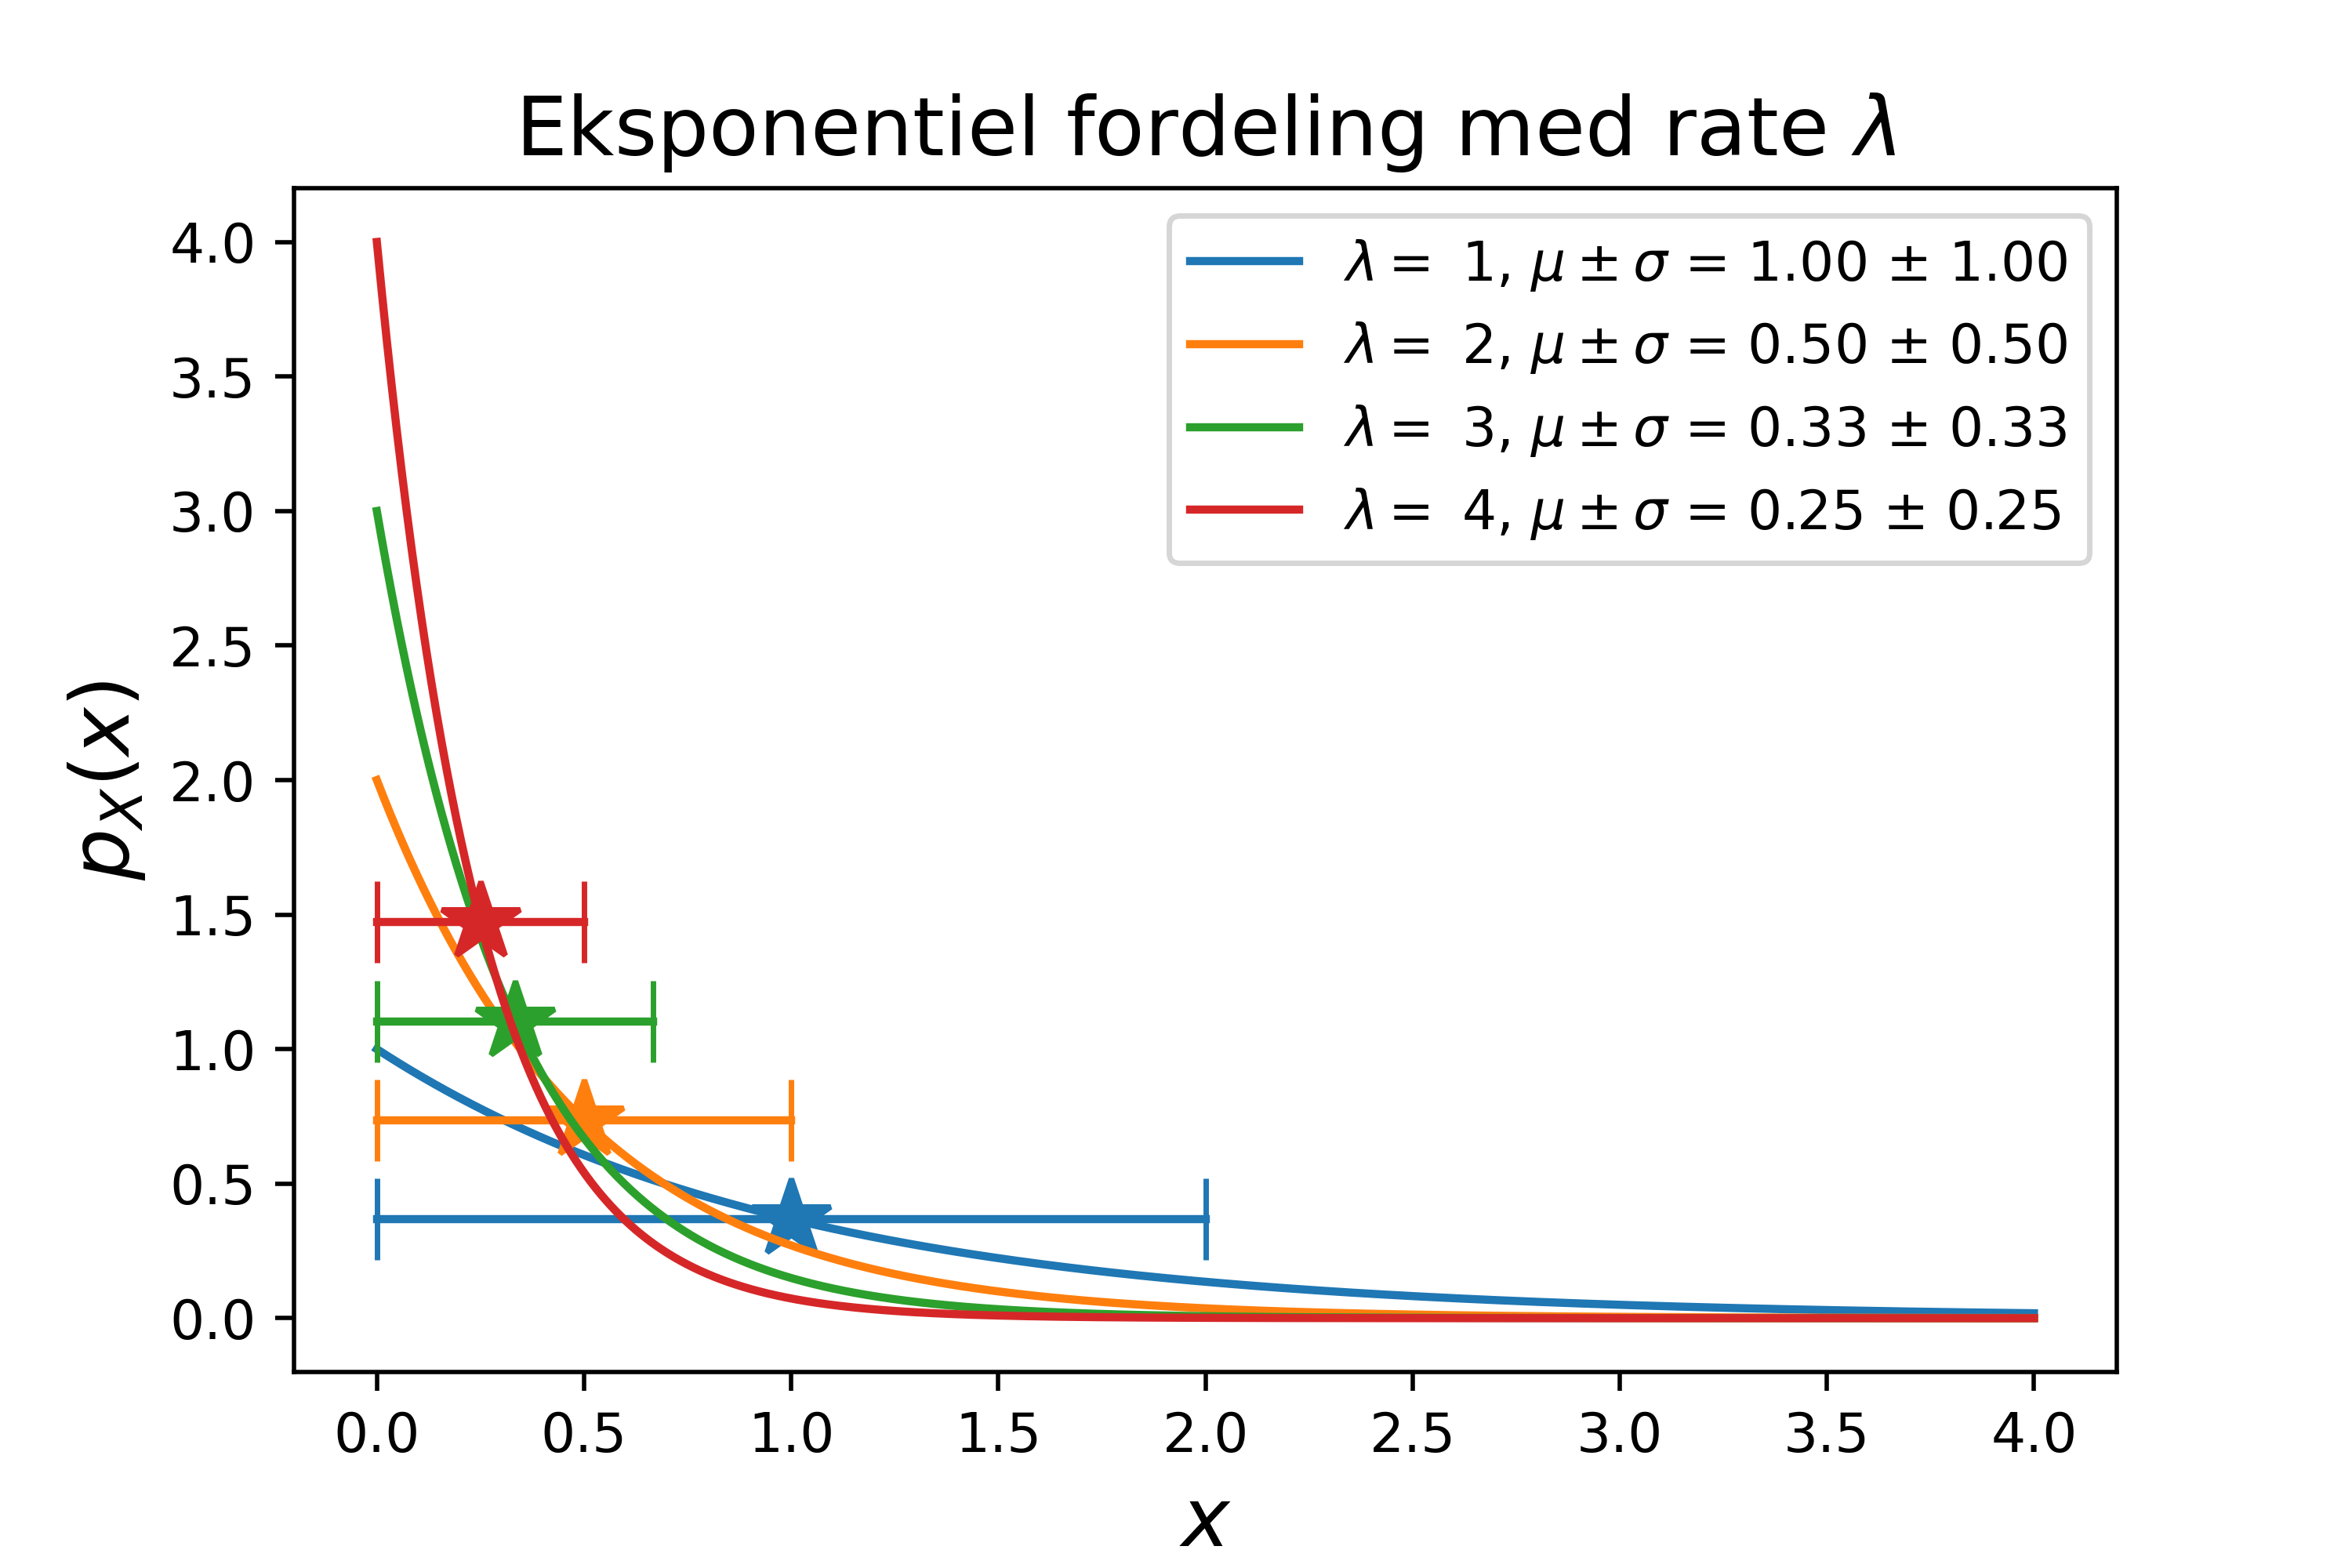
\includegraphics[width = \textwidth]{exp_dist.png}
\end{minipage}
\begin{minipage}[b][][b]{.45\textwidth}
\centering
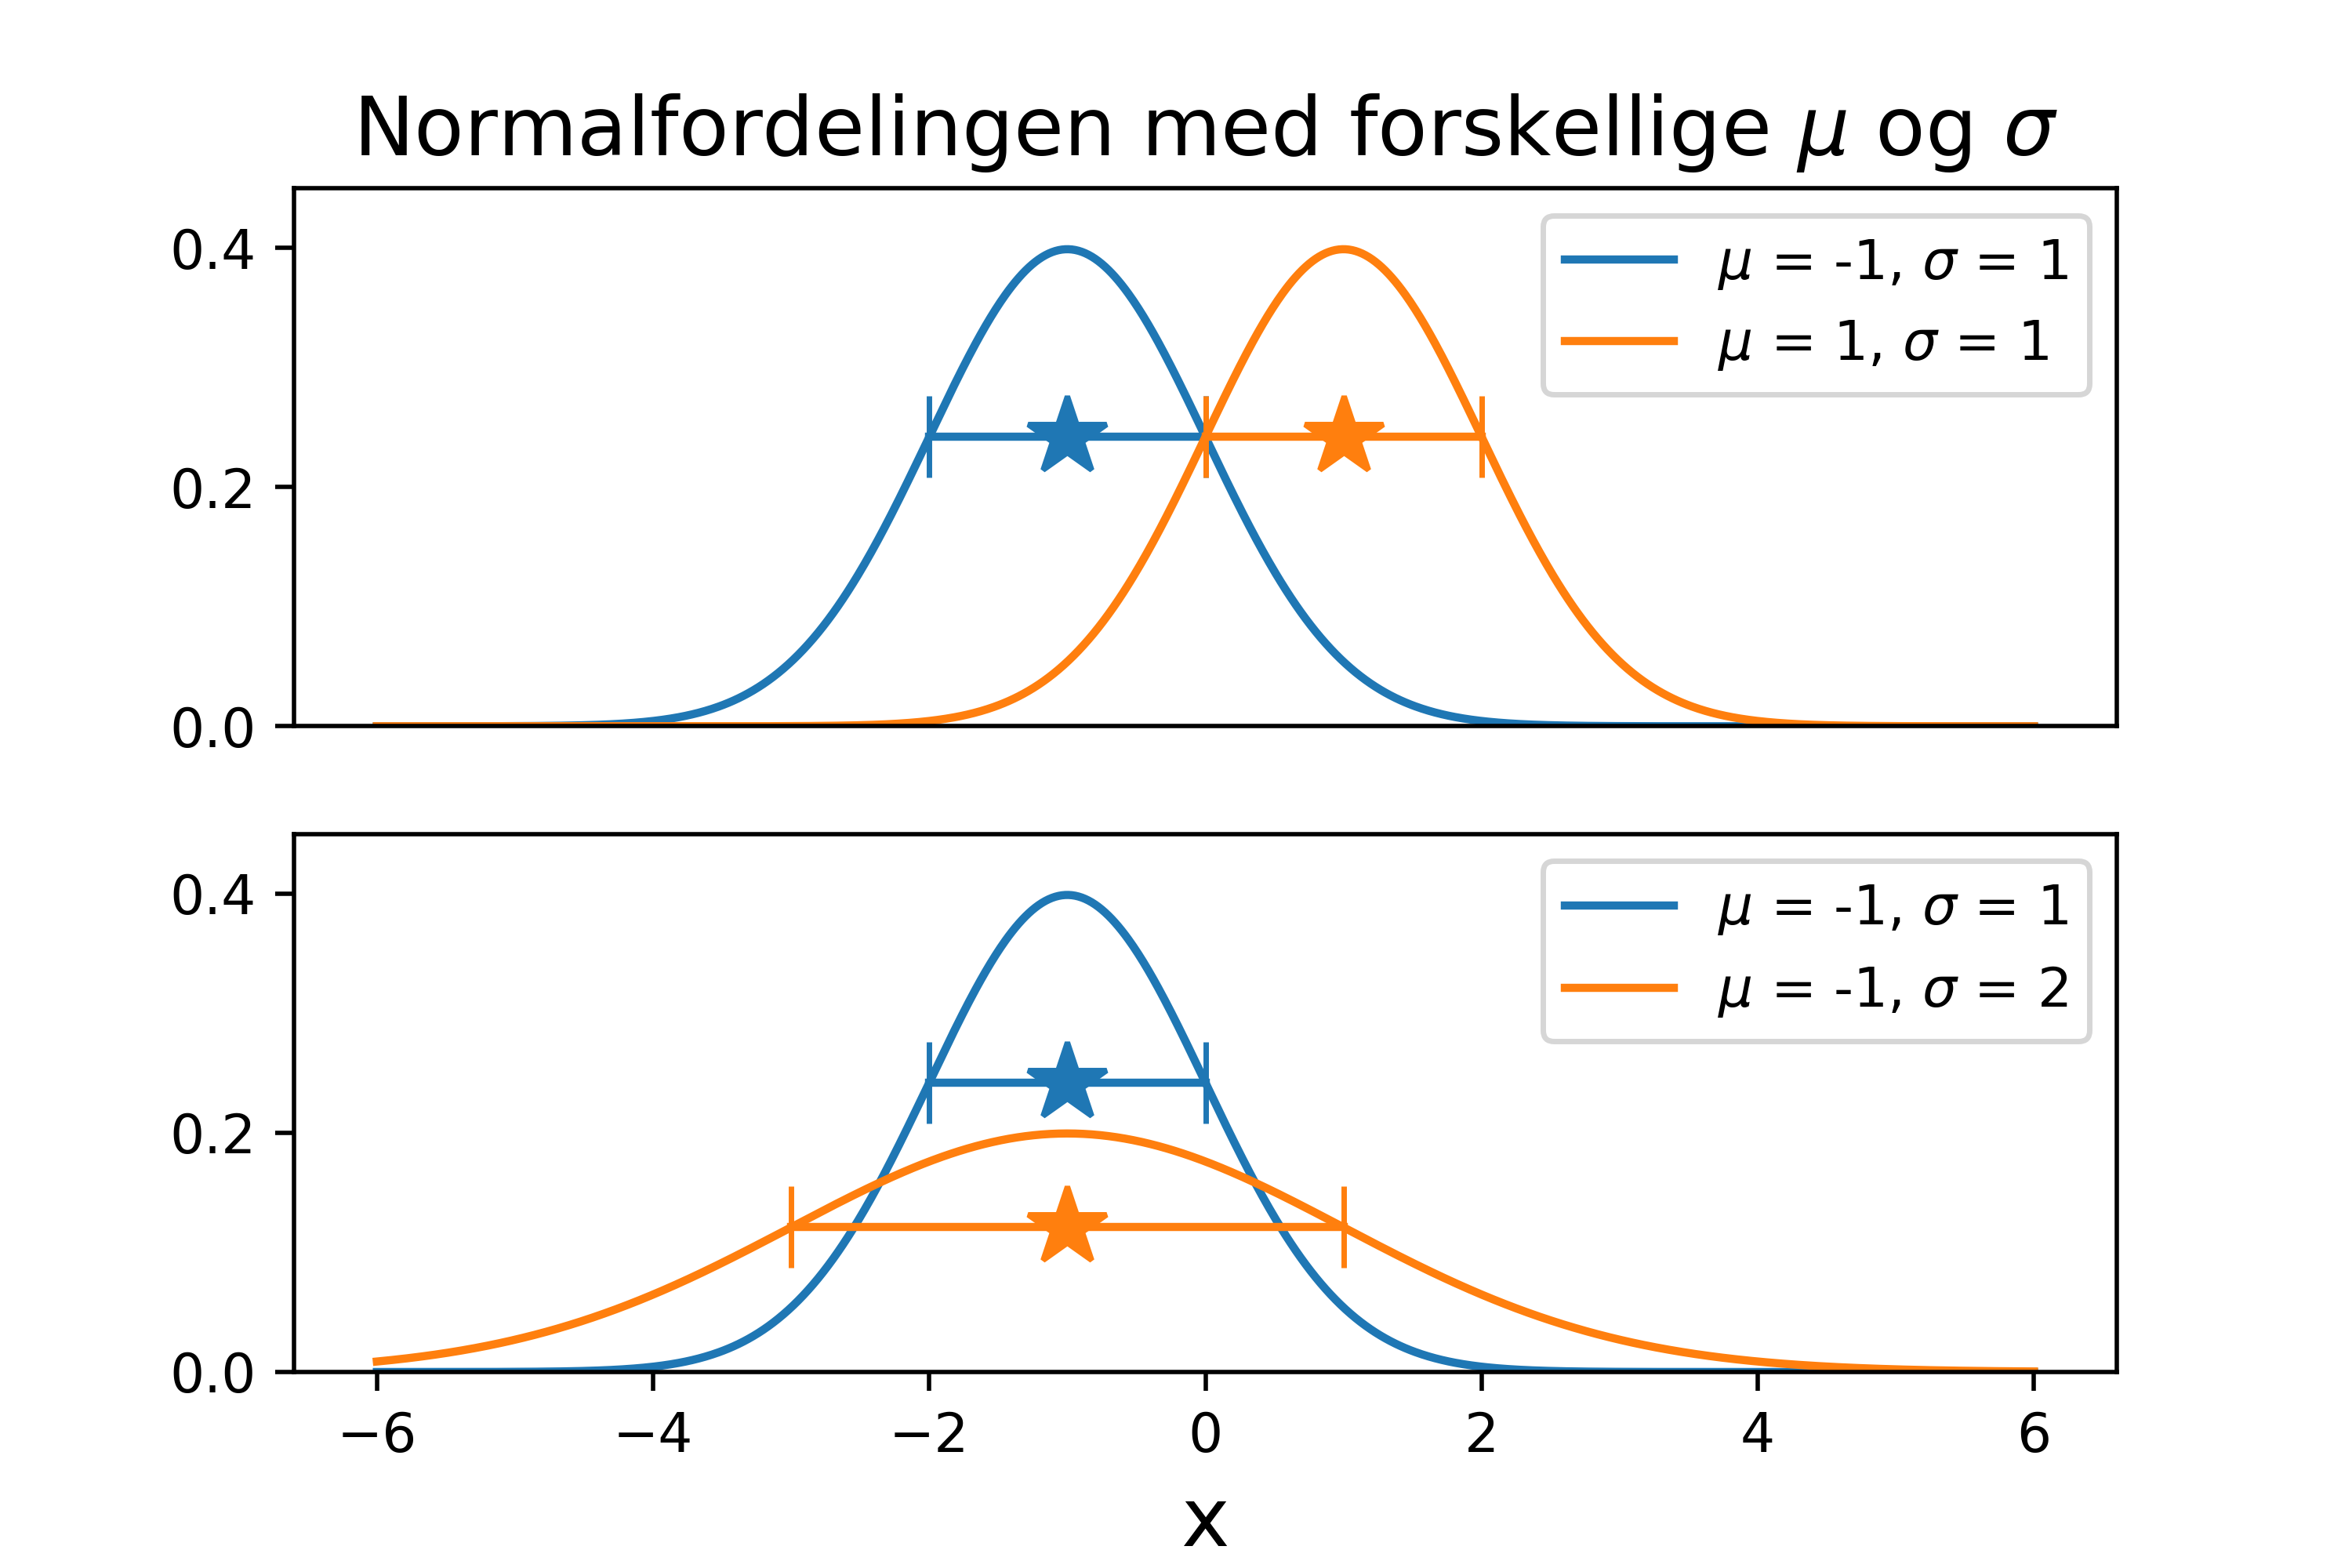
\includegraphics[width = \textwidth]{normal.png}
\end{minipage}
\caption{Eksponentiel og normal fordeling med forskellige parametre. Stjernerne og tilhørende intervaller er forventet værdi $\mu$ $\pm$ standardafvigelse $\sigma$.} \label{fig:expnorm}
\end{figure}
\subsection{Normalfordeling}
Sidst men ikke mindst har vi normalfordelingen. Normalfordelingen er en kontinuert tilfældig variabel, og er den mest brugte indenfor statistik. Den optræder eksempelvis ved støjen på en radiokanal, IQ for en befolkning, spændingen fra en strømforsyning og meget mere. Hvis man ikke kender til fordelingen for en tilfældig variabel vil statistikere ofte antage en normalfordeling.   Fordelingen opstår når der måles en størrelse hvor mange tilfældige faktorer og støj påvirker målingen. Fordelingen er karakteriseret ud fra dens forventede værdi $\mu$ og varians $\sigma^2$, og hvis $X$ følger en normalfordeling med $E[X] = \mu$ og $\Var[X] = \sigma^2$, da er pdf'en:
\begin{align*}
p_X(x) = \frac{1}{\sqrt{2\pi\sigma^2}}\cdot e^{\displaystyle-\frac{1}{2\sigma^2}(x-\mu)^2}, \quad  x \in \mR,
\end{align*}
og vi skriver $X \sim \mathcal{N}(\mu,\sigma^2)$. Se figur \ref{fig:expnorm} for hvordan $\mu$ og $\sigma^2$ har indflydelse på formen på pdf'en. Bemærk at normalfordelingen kan antage alle reelle tal $\mR$. En process hvor negative tal ikke er mulige, såsom vindhastighed, er derfor ikke altid godt modeleret med normalfordelingen især hvis den forventede værdi er tæt på $0$. Se \cite[127-131]{olofsson2012} for mere om normalfordelingen. 